\documentclass[a4paper, 11pt]{article}
\usepackage{comment} % enables the use of multi-line comments (\ifx \fi) 
\usepackage{lipsum} %This package just generates Lorem Ipsum filler text. 
\usepackage{fullpage} % changes the margin
\usepackage{graphicx}
\usepackage{caption}
\usepackage{subcaption}

\begin{document}
%Header-Make sure you update this information!!!!
\noindent
\large\textbf{Machine Learning Project report} \hfill \textbf{Jiyan PutYourLastNameHere} \\
\normalsize ML \hfill \textbf{Massimo Innocentini} \\
Dr. Norman Hendrich \\
TA: Philipp Ruppel \hfill Due Date: 30/06/2018

\section*{Introduction}
In the forest cover dataset the goal is to predict the type fo cover that a certain has based on the observation of the environment. The dataset provides multiple features like soil type, area elevation, distance from water as we described in the first report. We have 7 types of cover type and each row in the data frame is associated with only a single type, thus the problem is known as multi-class classification. The Kaggle competition website states that the model submitted is simply evaluated on the accuracy to classify the cover type on the test data, the value is returned as a percentage so 100\% is perfect accuracy and obviously 0\% the model is useless.

\section*{Data Preprocessing}
In order to apply predictive model to the data we had to process in few different ways. First of all as was mentioned in the first part the different features are quite imbalanced, hence a the MinMaxScaler() function of sklearn was applied on the data. This first step ensures that each data is a value between 0 and 1 and that each feature has the same weight during training.

The other two processes were applied to reduce the dimensionality of the data and extract further meaning out of the current features.  First we compressed the wilderness area and soil type into single columns \cite{skill} in order to reduce the size of the data frame. This means that we added a \texttt{Soil Type} column and a \texttt{Wilderness Area} column. After we tried to use common sense and the plots we had from the data exploration in order to find features which were not really unique. These process was refined with trial and error during training the models and at the end we maintain only the features which resulted in the best accuracy. The idea is that if a feature is not improving the accuracy of the model than It is simply slowing down the process.

However a remark to be made is that It may be possible that a feature is not characteristic of the training set but It is in the test data. Clearly there is not much we can do since the model would not be able to learn about it.So after few trial we eliminated quite few features and we had left: \texttt{Elevation}, \texttt{Aspect}, \texttt{Wilderndess Area}, \texttt{Soil Type}, which were also the one we identified from the plots during the exploration of the data.

The final preprocessing of the data was done following the Kernel from Lathwal \cite{code}, which decided to pull the different features together and extract a metric to describe them in correlation to each other. The resulting extra columns were: 
\begin{itemize}
  \item \texttt{Slope Hydrology}: Describes the correlation between the horizontal and vertical distance from water source.
  \item \texttt{Mean Fire Hydrology|}: Describes the average distance from fire points and the respective water source.
  \item \texttt{Mean Amenities}: Describes the average distance from fire points, water and roadways.
  \item \texttt{HF1, HF2}: Indicates sum and difference distance from water source and fire points.
  \item \texttt{HR1, HR2}: Indicates sum and difference distance from water source and roadways.
  \item \texttt{FR1, FR2}: Indicates sum and difference distance from fire points and roadways.
\end{itemize}
At the end the features used for training are the following:  \texttt{Elevation}, \texttt{Aspect}, \texttt{Wilderndess Area}, \texttt{Soil Type}, \texttt{Slope Hydrology}, \texttt{Mean Fire Hydrology|}, \texttt{Mean Amenities},  \texttt{HF1, HF2}, \texttt{HR1, HR2}. We also dropped \texttt{FR1, FR2} at the end because It was not contributing to the accuracy of the model.

In order to perform the training and testing the training provided by Kaggle was split into 80/20 for local training and testing. Kaggle does not provide the targets for its test data hence It would be too slow to always upload the code on the website to validate the model. Moreover the amount of submission are limited per day. Thus the validation and optimisation of the parameters is initially done locally on the 20\% left of the training data.

Finally It was worth mentioning that applying PCA and using N=3 for the components did not help the training and the accuracy was quite low compared to using the columns listed earlier.

\section*{kNN}
The first classifier that we tried was kNN. We know that kNN is susceptible to imbalances in the data and we wanted to investigate how much It would affect the accuracy. Fig \ref{knn_no_norm} and \ref{knn_norm} shows the  script testes the classifier with neighbours going from 1 to 20 and record the accuracy for each. In our case with K=3 we had the best results of close to 0.8\% on the partial training data used for testing. We uploade the script as a Kernel on Kaggle and tested it agains the test data and we scored 0.66\%. The KNN is a simple model so we the result were expected not to be great.

\begin{figure}[htb]
\centering
  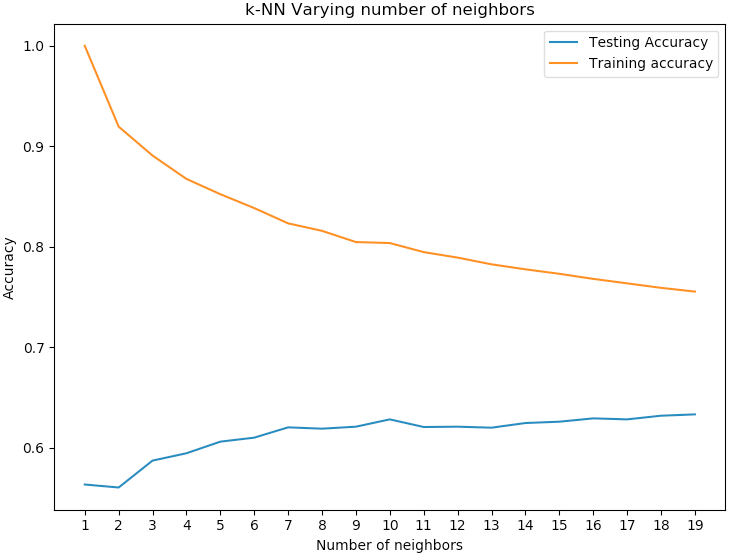
\includegraphics[width=1\textwidth]{img/knn_no_norm}
  \captionof{figure}{Applying KNN on  non-normalised data.}
  \label{knn_no_norm}
\end{figure}

\begin{figure}
\centering
  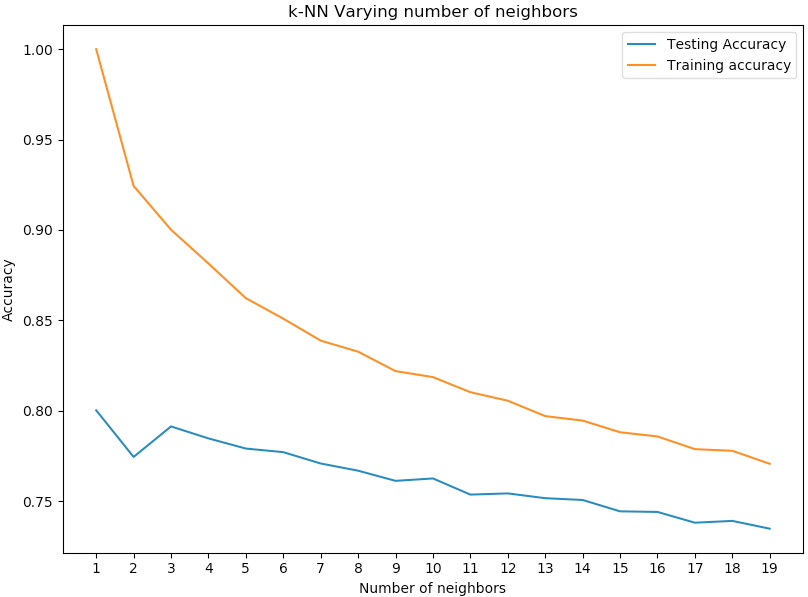
\includegraphics[width=1\textwidth]{img/knn_norm}
  \captionof{figure}{Applying KNN on normalised data.}
  \label{knn_norm}
\end{figure}

\section*{Neural Network}
After the KNN we decided to implement a deep neural network model by using Keras. We implemented a Multilayer perceptron (MLP) an input node, 2 hidden layers and a final output. Moreover in between each layer we use a dropout method for regularisation in order to avoid overfitting in the long run. The structure of the network takes as input the features we selected at the beginning and then connected to a 128 neurons hidden layer ReLU activation. The second hidden layer is identical to the first with another 128 neurons and ReLU activation. Finally the network outputs 7 values using a \texttt{softmax} activation.

Using a softmax function meant that the output of the network was actually a vector of 7 elements indicating the probability for each output. Thus the target on the training data and test data had to be encoded accordingly. The process is called hot one encoding and the module \texttt{np\_utils}, which as the method to transform the data can be imported from \texttt{keras.utils}.

The network uses a \texttt{categorical\_crossentropy} as function loss and the optimisation function used \texttt{adam}. We tried to \texttt{SGD} however we had better results with \texttt{adam}. The structure of the MLP was implemented as the Keras documentation presents. We trained the network using 100 epochs and a batch size of 128. The parameters were tested multiple times with different number of neurons, optimisers, epochs and batch size but the results obtained did not differ significantly. The major difference was that a network with less neurons or smaller batch size needed more epochs to produce the same results.

At the end we tested the network on the test data on the Kaggle website and even though we improved slightly, from 0.66\% to 0.69\% the results were still quite low.

\section*{ExtraTreesClassifier}
The other classifier used is an ensemble method called ExtraTreesClassifier which is the on used by Lathwal \cite{code}. The algorithm tries to fits multiple random decision trees on multiple sub-samples and tries to improve the average accuracy to find the best algorithm to predict the data. One downside of classifiers which use randomised trees is to optimise the number of trees to use, also referred to as estimators. For this reason we applied the same concept as with KNN and tested it with the number of estimators going from 50 to 1000 with steps of 50. The results are shown in Fig \ref{trees} and they show a way better accuracy compared to the other classifiers used. Moreover the results carryover on the real test data from Kaggle, which is the most important aspect, in fact on the Kaggle data the accuracy is equal to 0.80597\%, our best entry.

\begin{figure}
\centering
  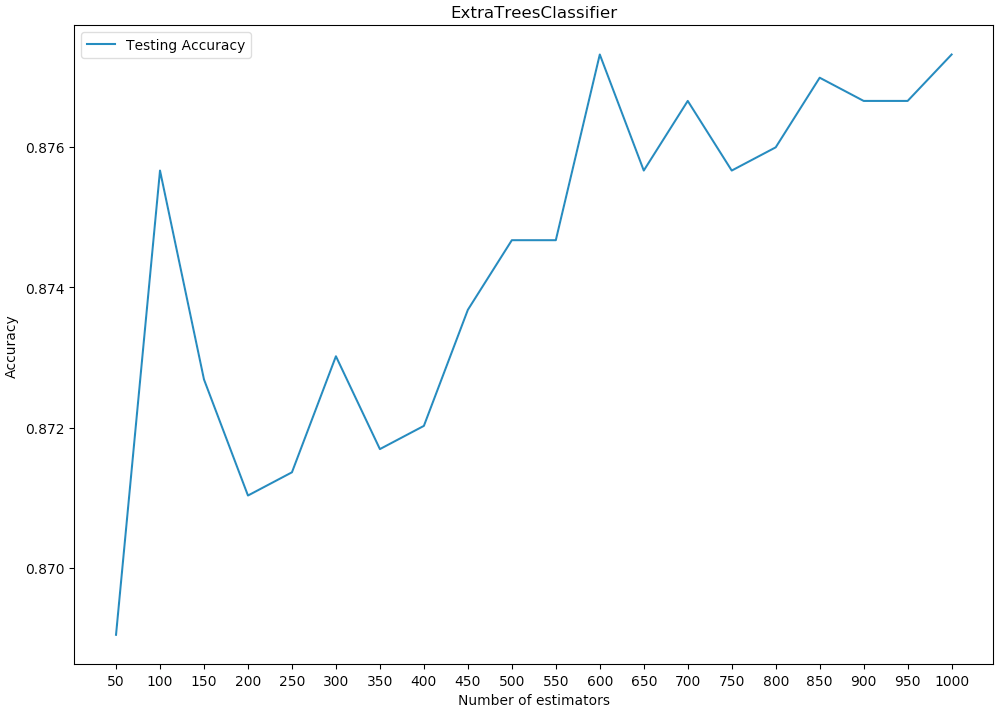
\includegraphics[width=1\textwidth]{img/extra_trees}
  \captionof{figure}{ExtraTreesClassifier performance on the local test data.}
  \label{trees}
\end{figure}

\section*{Support Vector Machine}

\section*{Discussion \& Comparison}
Comparing the different models used the ExtraTreesClassifier clearly showed the best result, moreover the time needed for training was quite short compared to all the other models. At the same time I think there is more to explore withe the MLP, more time is needed to tinker with the structure and other details. As of now I would recommend the ExtraTreesClassifier in cases where there is not a sub group of distinctive features in a data set.

In terms of result we would say for the small training data available the results are quite good, the test data consists of over half a million samples, while the training data is only 15k. Hence we feel there were quite few features which were underrepresented in the training set. It also means that the training set was composed of a subset of certain features, which made the model more prone to overfit. In addition we believe that the coordinates, or at least an identification of some kind, of the location and observations on the climate would have been a good addition to the data set.

\section*{Conclusion}
In conclusion It seems the ensemble method with the random trees performs the best, this is matches the result of the other public Kernels published in the competition since the most accurate models use decision trees. There is probably more work to do with the preprocessing of the data in order to use all the features in a meaningful way. We also think that the neural network model can perform much better than that with a more aimed structure and parameters. Finally It is helpful in this cases to do more research about the topic covered, for instance having more knowledge about botanic may highlight certain details which did not seem important at the beginning.

\begin{thebibliography}{9}
\bibitem{code} Lathwal. https://www.kaggle.com/codename007/forest-cover-type-eda-baseline-model
\bibitem{skill} Skillsmuggler. https://www.kaggle.com/skillsmuggler/eda-and-dimension-reduction
\end{thebibliography}

\end{document}